\newpage
\hypertarget{schema tex}{}
\subsection{Text Schema}
\texHeader

% Expand the crap outta all of this!

\begin{itemize}

\item[$\blacktriangleright$] Right-click on \texttt{MyWorkingSet}, and navigate to ``New / TGG'' (Fig.~\ref{fig:contextTGG}).

\begin{figure}[htbp]
\begin{center}
  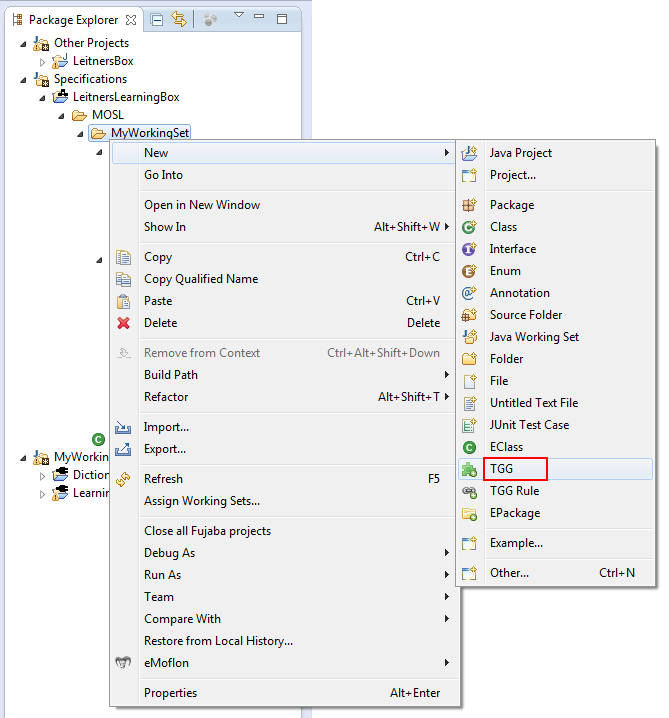
\includegraphics[width=0.8\textwidth]{eclipse_contextNewTGG}
  \caption{figureCaption}
  \label{fig:contextTGG}
\end{center}
\end{figure}

\item[$\blacktriangleright$] Name it \texttt{LearningBoxToDictionaryIntegration}, setting the source as \texttt{LearningBoxLanguage} and the target as
\texttt{DictionaryLanguage} (Fig.~\ref{fig:newTGG}).

\begin{figure}[htbp]
\begin{center}
  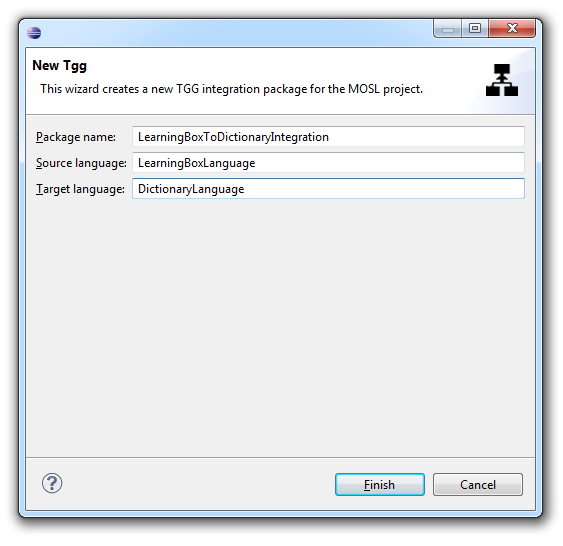
\includegraphics[width=0.9\textwidth]{eclipse_newTGG}
  \caption{figureCaption}
  \label{fig:newTGG}
\end{center}
\end{figure}

\item[$\blacktriangleright$] A new \texttt{schema} file should now be active in the editor! This is the \emph{TGG Schema} which declares ever
\emph{correspondence type} as \texttt{integration class}es. Press \texttt{ctrl + space} and use the auto completion to generate a new class template. \update
review the thesis : get the right names

\item[$\blacktriangleright$] Press \texttt{tab} to jump to each element, naming the class \texttt{BoxToDictionary}, and listing the source as \texttt{Box}
and target as \texttt{Dictionary} (Fig.~\ref{fig:newTGG}). We have set these objects this way as they are each containers which hold the smaller \texttt{card}
and \texttt{Entry} objects. In essence, these are the containers all new objects will be connected to.

\begin{figure}[htbp]
\begin{center}
  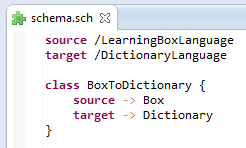
\includegraphics[width=0.4\textwidth]{eclipse_schemaFirstClass}
  \caption{figureCaption}
  \label{fig:firstCorrType}
\end{center}
\end{figure}

\item[$\blacktriangleright$] That's it! Your schema is now complete with connections to your \texttt{source} and \texttt{target} metamodels via a correspondence
link. To see how this is done in the visual syntax, check out Fig.~\ref{fig:firstCorrType} from the previous section.

\end{itemize}
